\chapter{非线性偏微分方程的精确解及其基础算法}
\section{Introduction}\label{Introduction-01}
In recent years, nonlinear evolution equations (NLEEs) have attracted particular attention from mathematicians, physicists and engineers. There are varieties of methods to construct exact solutions of NLEEs, such as the Inverse Scattering Method \cite{kawata1978inverse,ma2014verifying}, Darboux transformation method \cite{matveev1991darboux,ling2018general,lou1997non}, B{\"a}cklund transformation method \cite{wahlquist1973backlund,li2008method,cheng2015multiple}, Hirota bilinear method \cite{hirota1971exact,hereman1991exact,hu2002application,hirota2003vector,ma2015lump} and Wronskian technique \cite{freeman1983soliton,ito1988reduce,wu2008n}, etc. By using such varieties of schemes, several kinds of exact solutions are obtained, such as solitons \cite{hirota1971exact,makhankov1980computer}, breathers \cite{tajiri1989breather,guo2011rogue,sun2018general}, lump solutions \cite{satsuma1979two,villarroel1999discrete,imai1997dromion}, rogue waves \cite{guo2011rogue,zhang2014rogue,sun2018general,zhaqilao2018symbolic}, and so on.

Hirota bilinear method \cite{hirota1971exact}, which was proposed in 1971, plays an important role in the solving of NLEEs. Especially, the Hirota method is usually applied to construct soliton solutions of NLEEs. With the obtained soliton solutions, we can further calculate breather and lump solutions by the conjugate parameter assignment \cite{tajiri1989breather} and long wave limit \cite{satsuma1979two} method, respectively. These three methods are all algebraic methods to be easily algorithmized and implemented in mathematical softwares, such as, Maple, Mathematica, etc. This paper aims to algorithmize these methods and  implement automated derivation of soliton, breather and lump solutions for (n+1)-dimensional NLEEs.


We should note that the well known formula of n-soliton solution works well for integrable systems, but for non-integrable systems, such as (3+1)KP\CITEcaKP, (3+1)JM\CITEcaJM{} and (3+1)BKP\CITEcaBKP{} equations, it fails. Through a lot of experiments, we found that under appropriate parameters constraints, the false solution (the solution does not meet the original equation) becomes to be genuine solution (the solution meet the original equation). Moreover, the representation of generating formula of m-solitons or m-lumps is not friendly for programming. In order to derive these solutions automatically, these formulas have been properly modified by us in our algorithm for better programming and generalization.

The paper is organized as follows. In \refsec{Method-01}, our algorithm is expounded and an example is given to illustrate the key steps of our algorithm. \refsec{Implementation-01} introduces some details about the implementation and usage of our package. In \refsec{Examples-01}, we apply our program to some examples to illustrate the effectiveness. At the same time, we point out some practical techniques of extending our algorithm to higher dimensional equations. Finally, conclusions are given in \refsec{Conclusions-01}. 

\section{The description  of our algorithm}\label{Method-01}
In our algorithm, we first calculate soliton solutions by the simplified Hirota method, in which the transformation is derived from the standard truncated \Painleve{} expansion.  Then on the basis of the obtained soliton solutions, we further calculate breather and lump solutions by the conjugate assignment  and long wave limit method, respectively. For the convenience to implement these methods, we have adopted new representation for some key steps in the algorithm.  

\subsection{The transformation established from truncated \Painleve{} expansion}
In general, for the (n+1)-dimensional undetermined function $u=u(x_1,\cdots,x_n,t)$, a NLEE of it is a polynomial w.r.t. $u$ and its derivatives, i.e.,
\begin{equation}
    U(u,u\up{1},u\up{2},u\up{3}\cdots)=0. \label{oeq}
\end{equation}
Here, $u\up{k}~(k=1,2,3,\cdots)$ means all $k$ order derivatives with respect to its independent variables. For example, $u\up{1}=\bbrace{u_t,u_{x_1},\cdots,u_{x_n}}$ and $u\up{2}=\bbrace{u_{t,x_1},\cdots,u_{t,x_n},u_{x_1,x_2},\cdots}$.

Assuming \refeqn{oeq} admits the TPE (truncated \Painleve{} expansion) \cite{xu2004symbolic,xu2009note}
\begin{equation}
    u=\frac{1}{f^\alpha}\sum_{k=0}^{\alpha-1}{u_k(x_1,\cdots,x_n,t) f^k}, \label{tr}
\end{equation}
where $f=f(x_1,\cdots,x_n,t)$, and $\alpha$ can be determined by the principle of homogeneous balance \cite{wang1995solitary,wang1996application}. When $\alpha$ was determined, substitute \refeqn{tr} into \refeqn{oeq}, letting coefficients for different powers of $1/f$ to be zero, which is used to solve $u_k$. If each $u_k$ can be solved, substituting them into \refeqn{tr} gives us the desired transformation, otherwise the algorithm will terminate.

Actually, TPE is a generalization of logarithmic transformation. For example,  
\begin{equation}
    u=R[\ln(f)]_x=R\frac{f_x}{f} \text{~~and~~} u=R[\ln(f)]_{xx}=R\sbrace{\frac{f_{xx}}{f}-\frac{f_x^2}{f^2}}
\end{equation}
are in the form of \refeqn{tr}. 

Substitute the obtained transformation into the original \refeqn{oeq} and take the numerator, we get an equation with respect to $f$ and its derivatives, i.e.,
\begin{equation}
    F(f,f\up{1},f\up{2},f\up{3}\cdots)=0. \label{feq}
\end{equation}

\subsection{The simplified Hirota method for constructing soliton solutions}
Hirota bilinear method is an effective method to construct soliton solutions for NLEEs. However, we found that some NLEEs don't possess bilinear form. To bypass bilinear form the simplified Hirota method was proposed, which can be used to solve more wide range of NLEEs. We apply the simplified Hirota method to construct soliton solutions for NLEEs. In addition, m-soliton solutions for non-integrable systems could be established from the formula of m-soliton solution by appropriate parameters constraints. Our algorithm also works well for non-integrable systems. The process of the simplified Hirota method in our algorithm is described as follows.

Assuming $f$ is a function with respect to the travelling wave variable
\begin{equation}
    \xi=p_1\sbrace{x_1+p_2x_2+\cdots+p_nx_n+\omega t}+p_{n+1}. \label{tw}
\end{equation}
Here, $PL=\mbrace{p_1,p_2,\cdots,p_{n+1}}$ is the list of parameters. For example,  
\begin{equation}
    \xi=k(x+py+qz+\omega t)+c.
\end{equation}
Let
\begin{equation}
    f=1+\exp\sbrace{\xi}, \label{1-soliton}
\end{equation}
substitute it into \refeqn{feq} and solve the dispersion relation $\omega$. For an expression $e$ that contains $p_i~(i=1,\cdots,n+1)$, we define a \emph{subscript mapping function}
\begin{equation}
    S(e,k): \left\{\begin{array}{ll}
        p_i \rightarrow p_{i,k} & i \in \PS, \\ 
        p_i \rightarrow p_i & i \not\in \PS.
    \end{array}\right.
\end{equation}
Here, $\PS$ is the \emph{index set of parameters}, and 
\begin{equation}
    \PS\subseteq  \ALLP=\bbrace{1,2,\cdots,n,n+1}.
\end{equation}
In this paper, $\subseteq$ means subset, and $\subsetneq$ means proper subset. Then, substitute
\begin{equation}
    f=1+\exp\sbrace{\xi_i}+\exp\sbrace{\xi_j}+h_{i,j}\exp\sbrace{\xi_i+\xi_j} \label{hij}
\end{equation}
into \refeqn{feq} and solve the interaction coefficient $h_{i,j}$. Here, $\xi_i=S(\xi,i)$, $\xi_j=S(\xi,j)$.

When $\omega$ and $h_{i,j}$ were solved, we could calculate soliton solutions. Otherwise, our algorithm will terminate and output error information. The equation that can obtain $\omega$ and $h_{i,j}$ by our algorithm is called solvable. Otherwise, it is called insolvable.

It should be noted that, $\PS$ is critical in our algorithm. $\PS= \ALLP$ means an n-soliton solution expressed by the well known formula without any parameters constraints for an (n+1)-dimensional equation. The reasons why we introduce $\PS$ is shown below.
\begin{compactenum}[1. ]
\item For some non-integrable equation, when taking $\PS= \ALLP$ will get false solution, but when taking $\PS\subsetneq  \ALLP$ will get genuine solution.
\item Although, $\PS\subsetneq  \ALLP$ can be regarded as the special case of $\PS= \ALLP$. For some equations, we cannot calculate $h_{i,j}$ when $\PS= \ALLP$.
\item For non-integrable systems, we found that the obtained soliton solutions meet the original equation when forcing $p_{i,k}~(k=1,2,\cdots,m)$ have the same value.
\end{compactenum}
We will illustrate these points in the later example in this paper.

The well-know formula of m-soliton solution is \cite{hirota1973exact}
\begin{equation}
    f_{m-soliton}=\sum_{\mu=0,1}\exp\sbrace{\sum_{i=1}^m{\mu_i \xi_i}+\sum_{1\le i<j\le m}{\mu_i\mu_jH_{i,j}}}. \label{f-soliton-old}
\end{equation}
Here, the summation subscript $\mu=0,1$ means sum over all possible values. In fact, it sums over $\sbrace{\mu_1,\cdots,\mu_m}\in \bbrace{0,1}^m$. For example, 
\begin{equation}
\begin{split}
f_{3-soliton}&=1+\exp(\xi_1)+\exp(\xi_2)+\exp(\xi_3)\\
&+h_{1,2}\exp(\xi_1+\xi_2)+h_{2,3}\exp(\xi_2+\xi_3)+h_{1,3}\exp(\xi_1+\xi_3)\\
&+h_{1,2}h_{2,3}h_{1,3}\exp(\xi_1+\xi_2+\xi_3).
\end{split}
\end{equation}
Here, $h_{i,j}=\exp(H_{i,j})$.

The formula of m-soliton solution firstly comes up in the original paper of Hirota method in \cite{hirota1971exact} with a different form. The form of \refeqn{f-soliton-old} was first proposed in \cite{hirota1973exact} and is widely accepted by other researchers. But we think it is confusing and not friendly for programming. So, we rewrite it as follows:
\begin{equation}
    f_{m-soliton}=\sum_{P\subseteq M}\mbrace{\sbrace{\prod_{\bbrace{i,j}\subseteq P}{h_{i,j}}}\exp\sbrace{\sum_{k\in P}{\xi_k}}}. \label{f-soliton-new}
\end{equation}
Here, $M=\bbrace{1,2,\cdots,m}$ and $\xi_k=S(\xi,k)$. Obviously, \refeqn{f-soliton-new} is equivalent to \refeqn{f-soliton-old}, and \refeqn{f-soliton-new} is more convenient for programming.

\subsection{The conjugate parameter assignment for constructing m-breather solutions}
On the basis of (2m)-soliton solutions, we could further calculate m-breather solutions by the conjugate assignment method \cite{tajiri1989breather}. The idea of this method is very simple, just by assigning conjugate values for each pair of parameters in the travelling wave variables, in this way, the original (2m)-soliton solutions will convert into m-breather solutions. We simply describe the basic idea and procedure as follows. 

According to \cite{tajiri1989breather}, the generation function of m-breather solution is
\begin{equation}
    f_{m-breather}=\conj{f_{(2m)-soliton}}, \label{f-breather}
\end{equation}
where ${\rm conj}$ is the \emph{conjugate parameter substitution function}. It assumes 
\begin{equation}
    p_{i,j}=p_{i,j+m}^*,~(j=1,2,\cdots,m).
\end{equation}
Furthermore, it makes $\xi_{j}=\xi_{j+m}^*$. Such as, we take
\begin{equation}
\begin{split}
    p_{i,j}&=p_{i,j,RE}+I\cdot p_{i,j,IM}, \\ 
    p_{i,j+m}&=p_{i,j,RE}-I\cdot p_{i,j,IM},
\end{split}
\end{equation}
in which $I$ is the imaginary unit, and $p_{i,j,RE},p_{i,j,IM}$ are real constants. As a simple example of \refeqn{f-breather}, we take $m=1$, the obtained 1-breather solution is shown below.
\begin{equation}
\begin{split}
f_{1-breather}&=1+\exp(\xi_1)+\exp(\xi_2)+h_{1,2}\exp(\xi_1+\xi_2) \\ 
&=1+\exp(\xi_1)+\exp(\xi_1^*)+h_{1,2}\exp(\xi_1+\xi_1^*).
\end{split}
\end{equation}
It can be seen that 1-breather solution is derived from 2-soliton solution. Generally, m-breather solution is derived from (2m)-soliton solution.

\subsection{The long wave limit method for constructing m-lump solutions}
Using long wave limit method \cite{satsuma1979two}, we can get m-lump solution from the corresponding (2m)-soliton solution. The basic idea and procedure are shown below.

Let 
\begin{equation}
\begin{split}
    \xi_i&=k_i\sbrace{x_1+p_ix_2+\cdots+r_ix_n+\omega t}+\xi_i^{(0)},\\
    \eta_i&=\xi_i-\xi_i^{(0)}.
\end{split}
\end{equation}
The key of this method is to find the following expansions when $k_i\rightarrow 0$,
\begin{equation}
\begin{split}
    \exp(\eta_i)&=1+k_i \theta_i+o(k_i), \\ 
    h_{i,j}&=1+k_ik_jb_{i,j}+o(k_i^2+k_j^2),
\end{split} \label{lump-expansion}
\end{equation}
where the notation $o(f)$ is the Peano form of the remainder, i.e., $\lim_{f\rightarrow 0}[o(f)/f]=0$.

Take $\exp\sbrace{\xi_i^{(0)}}=-1$ and substitute \refeqn{lump-expansion} into the formula of (2m)-soliton solution, we can get an m-lump solution. For a 2-soliton solution, omit the remainder, we have
\begin{equation}
\begin{split}
\Theta_1&=1+\exp(\xi_1)+\exp(\xi_2)+h_{12}\exp(\xi_1+\xi_2) \\ 
&= 1+\exp(\xi_1)+\exp(\xi_2)+(1+k_1k_2b_{12})\exp(\xi_1+\xi_2) \\ 
&=(1+\exp(\xi_1))(1+\exp(\xi_2))+k_1k_2b_{12}\exp(\eta_1+\eta_2) \\ 
&=(1-(1+k_1\theta_1))(1-(1+k_2\theta_2))+k_1k_2b_{12} \\
&=k_1k_2(\theta_1\theta_2+b_{12}).
\end{split}
\end{equation}
Since $k_1k_2$ is a constant factor, and can be eliminated by the TPE. So the form of 1-lump solution is 
\begin{equation}
    \Theta_1=\theta_1\theta_2+b_{12}.
\end{equation}

Following the proof in \cite{satsuma1979two}, we can get the form of m-lump solution, i.e.,
\begin{equation}
\begin{split}
    \Theta_m&=\prod_{k=1}^{2m}\theta_k+\frac{1}{2}\sum_{i,j}{b_{i,j}}\prod_{J\neq i,j}{\theta_J}+\frac{1}{2! 2^2}\sum_{i,j,k,l}{b_{i,j}b_{k,l}}\prod_{J\neq i,j,k,l}{\theta_{J}}+\cdots \\
    &+\frac{1}{s!2^s}\sum_{i,j,\cdots,u,v}\underbrace{{b_{i,j}b_{k,l}\cdots b_{u,v}}}_{s}\prod_{J\neq i,j,\cdots, u,v}{\theta_J}+\cdots. \label{f-lump-old}
\end{split}
\end{equation}
For example,
\begin{equation}
\renewcommand{\t}[1]{\theta_{#1}}
\renewcommand{\b}[1]{b_{#1}}
\begin{split}
\Theta_2&=\t{1}\t{2}\t{3}\t{4}+\b{1,2}\t{3}\t{4}+\b{1,3}\t{2}\t{4}+\b{1,4}\t{2}\t{3}+\b{2,3}\t{1}\t{4}\\
&+\b{2,4}\t{1}\t{3}+\b{3,4}\t{1}\t{2}+\b{1,2}\b{3,4}+\b{1,3}\b{3,4}+\b{1,4}\b{2,3}.
\end{split}
\end{equation}

Now, we are going to find the expansions in \refeqn{lump-expansion}. Regard $\eta$ as a function w.r.t. $k$, we have 
\begin{equation}
\begin{split}
\exp(\eta(k))&=\exp(\eta(0))+\eta'(0)\exp(\eta(0))k+o(k)\\ 
&=1+\eta'(0)k+o(k). 
\end{split}
\end{equation}
So, 
\begin{equation}
\theta=\eval{\frac{\partial \eta}{\partial k}}{k=0}=\eval{\frac{\partial \xi}{\partial k}}{k=0}.
\end{equation}
Let $h_{i,j}=h(k_i,k_j)$, for the symmetry, we have $h(x,y)=h(y,x)$. In addition, take $k_2=0$ in the 2-soliton solution, we get a 1-soliton solution, so we have $h(k_1,0)=1$. Symmetrically, we have $h(0,k_2)=1$. Thus, we have $h(0,0)=1$ and
\begin{equation}
    h_x(0,0)=\eval{\frac{\partial}{\partial x}h(x,0)}{x=0}=0.
\end{equation}
Similarly, we have $h_y(0,0)=h_{xx}(0,0)=h_{yy}(0,0)=0$. Thereupon, the expansion of $h(x,y)$ at $(0,0)$ is 
\begin{equation}
\begin{split}
h(x,y)&=h(0,0)+h_x(0,0)x+h_y(0,0)y \\ 
&+\frac{1}{2}\mbrace{h_{xx}(0,0)x^2+2h_{xy}(0,0)xy+h_{yy}(0,0)y^2}+o(x^2+y^2) \\ 
&=1+h_{xy}(0,0)xy+o(x^2+y^2).
\end{split}
\end{equation}
Thus, we get 
\begin{equation}
    b_{i,j}=\eval{\frac{\partial^2}{\partial k_i\partial k_j}h_{i,j}}{k_i=0,k_j=0}.
\end{equation}
Finally, for the travelling wave variable in \refeqn{tw}, the key parameters of lump solutions are
\begin{equation}
\begin{split}
    \theta &= \eval{\frac{\partial \xi}{\partial p_1}}{p_1=0}, \\
    b_{i,j}&= \eval{\frac{\partial^2}{\partial p_{1,i}\partial p_{1,j}}h_{i,j}}{p_{1,i}=0,p_{1,j}=0}.
\end{split} \label{p-lump}
\end{equation}
\refeqn{p-lump} shows that lump solution requires $\bbrace{1}\subsetneq \PS$.

The generation function of m-lump solution is
\begin{equation}
    f_{m-lump}=\conj{\Theta_m}.
\end{equation}
Because \refeqn{f-lump-old} is mysterious and not friendly for programming, we are going to rewrite it. In \refeqn{f-lump-old}, we set the number of $b_{i,j}$ in an item to $s$, the summation should be divided by $s!2^s$. Divided by $2^s$ means $b_{i,j}=b_{j,i}$. Divided by $s!$ means that only one expression should be selected from the full permutation of $b_{i,j}$. 

From this observation, we can rewrite \refeqn{f-lump-old} as
\begin{equation}
    \Theta_m=\sum_{l=0}^m\sum_{s\in L(l)}\sbrace{\prod_{k=1}^l{b_{s_{2k-1},s_{2k}}}\prod_{p\not\in s}{\theta_p}}, \label{f-lump-new}
\end{equation}
where 
\begin{equation}
    L(l)=\bbrace{\sbrace{s_1, s_2, \cdots ,s_{2l}}\left|s_{2k}>s_{2k-1},s_{2k+1}>s_{2k-1},s_k\in \bbrace{1,\cdots,2l}\right.}.
\end{equation}
Thus, every item in \refeqn{f-lump-new} is uniquely determined by a sequence $\sbrace{s_1, s_2, \cdots ,s_{2l}}$. Here, $s_{2k}>s_{2k-1}$ ensures that $b_{i,j}=b_{j,i}$, and only one of them appears in the formula. Similarly, $s_{2k+1}>s_{2k-1}$ ensures that only one expression should be selected from the full permutation of $b_{i,j}$. 

Consequently, \refeqn{f-lump-new} is equivalent to \refeqn{f-lump-old}, and \refeqn{f-lump-new} is clearer than \refeqn{f-lump-old}. Further more, \refeqn{f-lump-new} has no redundant summation, it means that generating m-lump solution by \refeqn{f-lump-new} is faster than that by \refeqn{f-lump-old}. 

\subsection{An example of application}
In this subsection, we are going to give a typical example to demonstrate how our algorithm works. 

Consider the (3+1)JM equation \CITEcaJM,
\begin{equation}
    u_{xxxy}+3u_{xx}u_y+3u{x}u_{xy}+2u_{ty}-3u_{xz}=0. \label{JMEQ3}
\end{equation}
The order list of this equation is $\mbrace{\alpha+4,2\alpha+3,2\alpha+3,\alpha+2,\alpha+2}$. From $\alpha+4=2\alpha+3$, we get $\alpha=1$. Thus, the TPE of this equation is $u=u_0/f$. Substitute it into \refeqn{JMEQ3}, we get $u_0=2f_x$, and the TPE of \refeqn{JMEQ3} is 
\begin{equation}
u=\frac{2f_x}{f}. \label{JMEQ-tr}    
\end{equation}

Substitute \refeqn{JMEQ-tr} into \refeqn{JMEQ3} and take the numerator, we get an equation with respect to $f$ and its derivatives, i.e., 
\begin{equation}
\begin{split}
0=&2\,{f}^{2}f_{{{ txy}}}+{f}^{2}f_{{{ xxxxy}}}-3\,{f}^{2}f_{{{ xxz}}}-2\,ff_{{t}}f_{{{ xy}}}-2\,ff_{{{ tx}}}f_{{y}}-2\,ff_{{{ ty}}}f_{{x}}\\
-&4\,ff_{{x}}f_{{{ xxxy}}}+6\,ff_{{x}}f_{{{ xz}}}+3\,ff_{{{ xx}}}f_{{z}}+2\,ff_{{{ xxx}}}f_{{{xy}}}-ff_{{{ xxxx}}}f_{{y}}\\
+&4\,f_{{t}}f_{{x}}f_{{y}}+6\,{f_{{x}}}^{2}f_{{{ xxy}}}-6\,{f_{{x}}}^{2}f_{{z}}-6\,f_{{x}}f_{{{ xx}}}f_{{{ xy}}}+2\,f_{{x}}f_{{{ xxx}}}f_{{y}}. \label{JMEQ-feq}
\end{split}
\end{equation}

Take $\xi=k(x+py+qz+\omega t)+c$ and substitute it into \refeqn{1-soliton}, then substitute the result into \refeqn{JMEQ-feq}, we get the dispersion relation $\omega=(3q-k^2p)/(2p)$.

Let $\PS=\bbrace{1,2}$,
\begin{equation}
\begin{split}
\xi_i&=k_i\sbrace{x+p_iy+qz+\frac{3q-k_i^2p_i}{2p_i}t}+c, \\ 
\xi_j&=k_j\sbrace{x+p_jy+qz+\frac{3q-k_j^2p_j}{2p_j}t}+c.
\end{split} \label{JMEQ-xij}
\end{equation}
It should be noted that only $k$ and $p$ have subscripts, which are specified by the set $\PS$. Substitute \refeqn{JMEQ-xij} into \refeqn{hij}, then substitute the result into \refeqn{JMEQ-feq}, we get the interaction coefficient
\begin{equation}
    h_{i,j}=\frac{(k_ip_j(k_i-k_j)+q)p_i^2-p_ip_j(k_jp_j(k_i-k_j)+2q)+qp_j^2}{(k_ip_j(k_i+k_j)+q)p_i^2+p_ip_j(k_jp_j(k_i+k_j)-2q)+qp_j^2}.
\end{equation}
Then, after applying \refeqn{p-lump}, we have
\begin{equation}
\begin{split}
&\theta=\frac{2p^2y+(2qz+2x)p+3pq}{2p}, \\ 
&b_{i,j}=-\frac{2p_ip_j(p_i+p_j)}{q(p_i-p_j)}.
\end{split}
\end{equation}

Finally, based on these intermediate results, we can further calculate soliton, breather and lump solutions, successively. That is,
\begin{compactitem}[\textbullet]
\item Substituting $\omega$ and $h_{i,j}$ into \refeqn{f-soliton-new} generates soliton solutions. \reffig{jm:1-soliton}, \reffig{jm:2-soliton} and \reffig{jm:3-soliton} show 1-soliton, 2-soliton and 3-soliton solutions in turn. 
\item Substituting $\omega$ and $h_{i,j}$ into \refeqn{f-breather} generates breather solutions. \reffig{jm:1-breather}, \reffig{jm:2-breather} and \reffig{jm:3-breather} are 1-order to 3-order breather solutions successively.
\item Substituting $\theta$ and $b_{i,j}$ into \refeqn{f-lump-new} generates lump solutions. \reffig{jm:1-lump}, \reffig{jm:2-lump} and \reffig{jm:3-lump} are 1-order, 2-order and 3-order lump solutions, respectively. 
\end{compactitem}

\begin{figure}
\centering 
\subfigure[1-soliton \label{jm:1-soliton}]{
    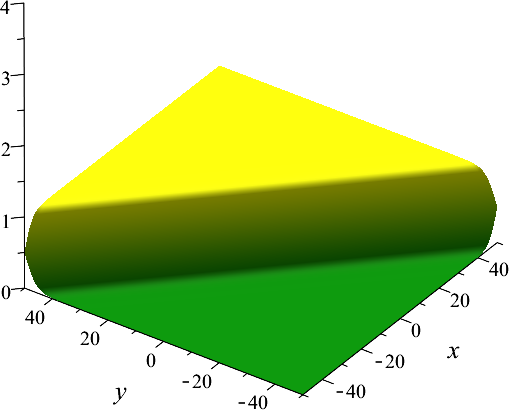
\includegraphics[width=.3\textwidth]{fig/(3+1)JM-1-soliton.png}    
}
\subfigure[2-soliton \label{jm:2-soliton}]{
    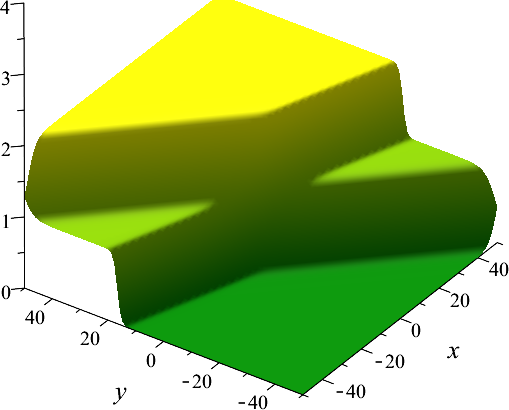
\includegraphics[width=.3\textwidth]{fig/(3+1)JM-2-soliton.png}
}
\subfigure[3-soliton \label{jm:3-soliton}]{
    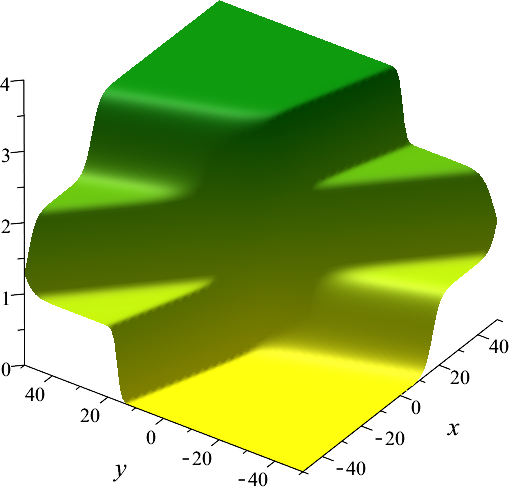
\includegraphics[width=.3\textwidth]{fig/(3+1)JM-3-soliton.png}
}
\subfigure[1-breather \label{jm:1-breather}]{
    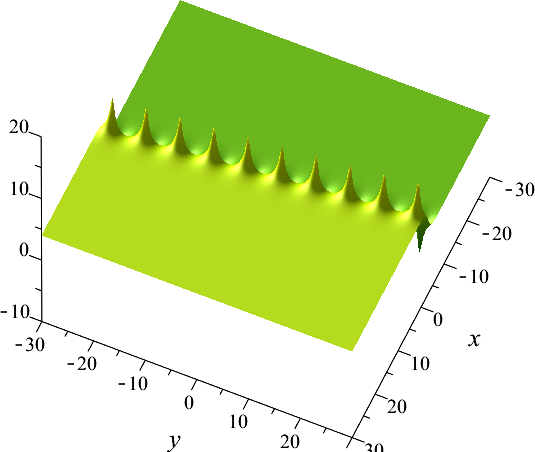
\includegraphics[width=.3\textwidth]{fig/(3+1)JM-1-breather.png}
}
\subfigure[2-breather \label{jm:2-breather}]{
    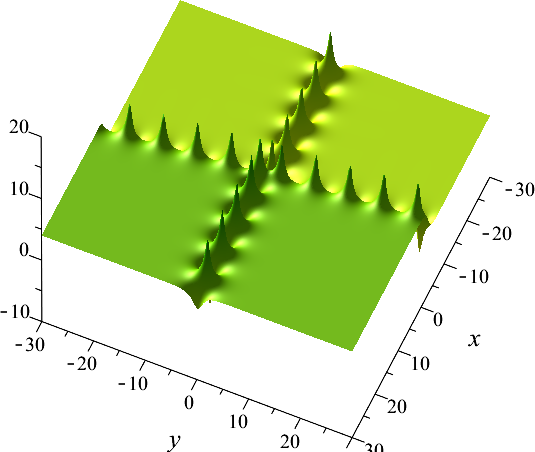
\includegraphics[width=.3\textwidth]{fig/(3+1)JM-2-breather.png}
}
\subfigure[3-breather \label{jm:3-breather}]{
    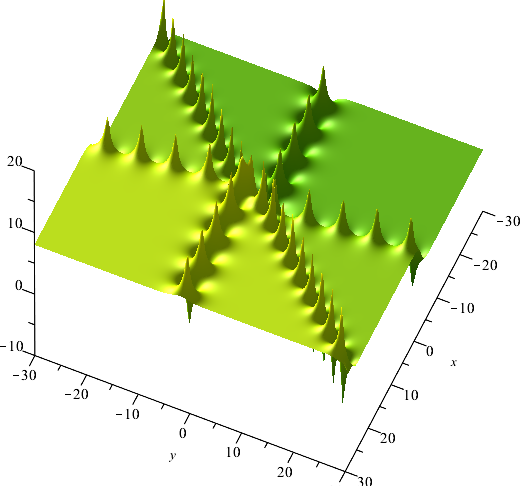
\includegraphics[width=.3\textwidth]{fig/(3+1)JM-3-breather.png}
}
\subfigure[1-lump \label{jm:1-lump}]{
    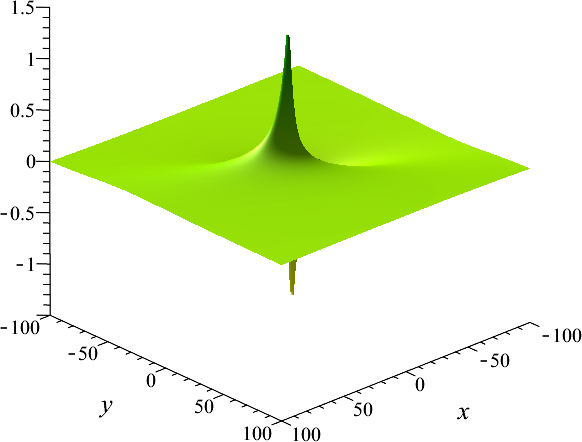
\includegraphics[width=.3\textwidth]{fig/(3+1)JM-1-lump.png}
}
\subfigure[2-lump \label{jm:2-lump}]{
    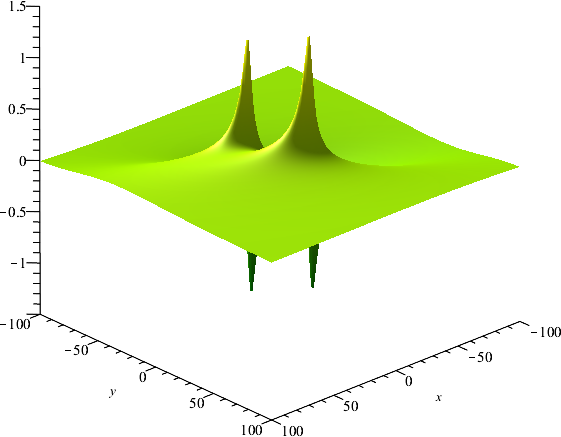
\includegraphics[width=.3\textwidth]{fig/(3+1)JM-2-lump.png}
}
\subfigure[3-lump \label{jm:3-lump}]{
    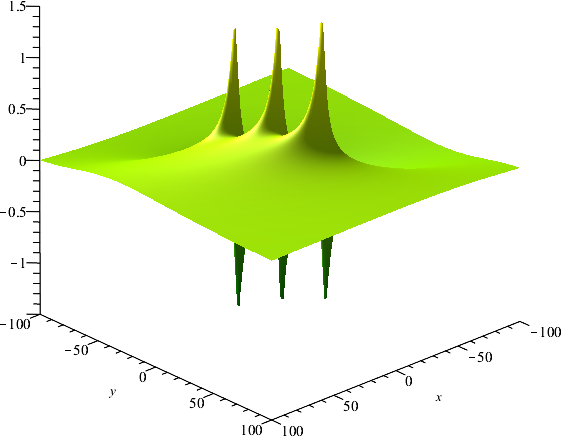
\includegraphics[width=.3\textwidth]{fig/(3+1)JM-3-lump.png}
}
\caption{Solutions of (3+1)JM equation}
\label{jm}
\end{figure}

It's very interesting that the breather solution shown in \reffig{jm:1-breather} is drawn w.r.t. independent variables $x,y$, but when drawing the same solution w.r.t. independent variables $x,z$, it appears as a periodic line wave as shown in \reffig{jm:1-periodic}. In addition, for a 2-breather solution, when setting parameters in one of the 2-breather to be real constants, and the parameters in another breather are still complex constants, then we get the interaction of a 1-soliton and a 1-breather as shown in \reffig{jm:soliton-breather}. 

\begin{figure}
\centering
\subfigure[1-periodic line wave \label{jm:1-periodic}]{
    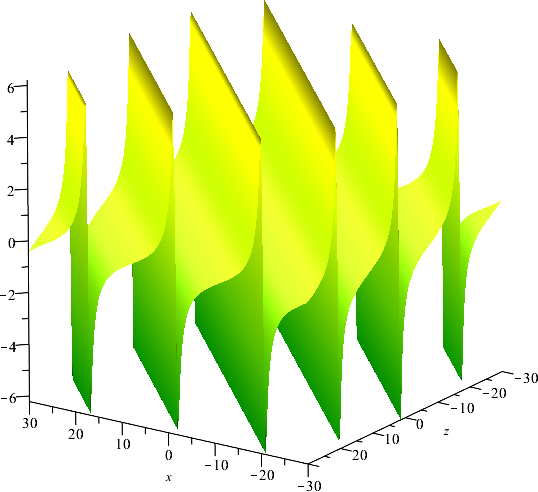
\includegraphics[width=.4\textwidth]{fig/(3+1)JM-1-periodic.png}
}
\subfigure[soliton-breather \label{jm:soliton-breather}]{
    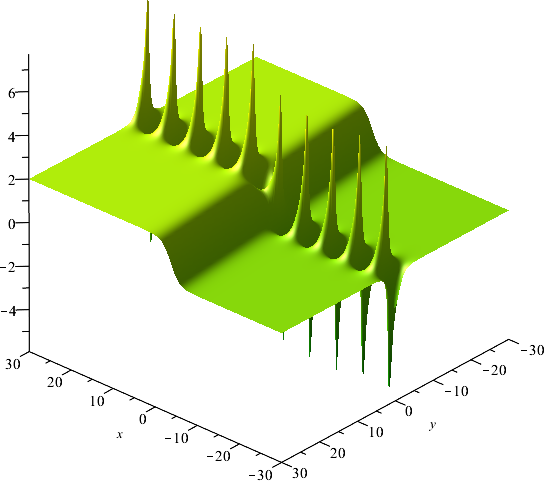
\includegraphics[width=.4\textwidth]{fig/(3+1)JM-soliton-breather.png}
}
\caption{Degenerated solutions of (3+1)JM equation} \label{jmd}
\end{figure}

The plotting parameters of \reffig{jm} and \reffig{jmd} are listed in \reftab{jm-plist}.

\begin{table}
\centering 
\caption{Plotting parameters in Figures \ref{jm},\ref{jmd} \label{jm-plist}}
\small
\renewcommand{\arraystretch}{1.1}
\begin{tabular}{cp{0.88\textwidth}}
\hline 
Fig. & \multicolumn{1}{c}{Plotting parameters} \\ 
\hline 
\ref{jm:1-soliton} & \texttt{{c=0, q=1, t=0, x=-50..50, y=-50..50, z=0, k[1]=1/2, p[1]=1}} \\
\ref{jm:2-soliton} & \texttt{{c=0, q=1, t=0, x=-50..50, y=-50..50, z=0, k[1]=1/2, k[2]=1/2, p[1]=1, p[2]=3}} \\
\ref{jm:3-soliton} & \texttt{{c=0, q=1, t=0, x=-50..50, y=-50..50, z=0, k[1]=1/2, k[2]=1/2, k[3]=1/2, p[1]=1, p[2]=3, p[3]=1/3}} \\
\ref{jm:1-breather} & \texttt{{c=0, q=1, t=0, x=-30..30, y=-30..30, z=0, k[1,IM]=0, k[1,RE]=1, p[1,IM]=1, p[1,RE]=1/10}} \\
\ref{jm:2-breather} & \texttt{{c=0, q=1, t=0, x=-30..30, y=-30..30, z=0, k[1,IM]=0, k[1,RE]=1, k[2,IM]=1, k[2,RE]=0, p[1,IM]=1, p[1,RE]=1/10, p[2,IM]=1, p[2,RE]=1/10}} \\
\ref{jm:3-breather} & \texttt{{c=0, q=1, t=0, x=-30..30, y=-30..30, z=0, k[1,IM]=0, k[1,RE]=1, k[2,IM]=1, k[2,RE]=0, k[3,IM]=1, k[3,RE]=1, p[1,IM]=1, p[1,RE]=1/10, p[2,IM]=1, p[2,RE]=1/10, p[3,IM]=1, p[3,RE]=1/10}} \\
\ref{jm:1-lump} & \texttt{{q=1, t=0, x=-100..100, y=-100..100, z=0, p[1,IM]=1, p[1,RE]=1}} \\
\ref{jm:2-lump} & \texttt{{q=1, t=0, x=-100..100, y=-100..100, z=0, p[1,IM]=1, p[1,RE]=1, p[2,IM]=1, p[2,RE]=6/5}} \\
\ref{jm:3-lump} & \texttt{{q=1, t=0, x=-100..100, y=-100..100, z=0, p[1,IM]=1, p[1,RE]=1, p[2,IM]=1, p[2,RE]=6/5, p[3,IM]=1, p[3,RE]=4/5}} \\
\ref{jm:1-periodic} & \texttt{{c=0, q=1, t=0, x=-30..30, y=0, z=-30..30, k[1,IM]=1/3, k[1,RE]=0, p[1,IM]=1, p[1,RE]=1/10}} \\
\ref{jm:soliton-breather} & \texttt{{c=0, q=1, t=0, x=-30..30, y=-30..30, z=0, k[1,IM]=1, k[1,RE]=0, k[2,IM]=0, k[2,RE]=1, p[1,IM]=1, p[1,RE]=1/10, p[2,IM]=0, p[2,RE]=1/10}} \\

\hline
\end{tabular}
\end{table}

\section{Implementation and demonstration}\label{Implementation-01}
Based on the description above, we implement the algorithm in Maple. In this section, we briefly introduce the interfaces and parameters of our program.

The implemented Maple package is named as \texttt{TwSolver}. The main interface of this package is 
\begin{verbatim}
sh:=twsolve(eq,PS,{PL,select_solution}).
\end{verbatim}
Here, parameters in \verb|{}| mean optional. These parameters are described as follows: 
\begin{compactitem}[\textbullet]
\item \texttt{eq} means the input equation in the form of \refeqn{oeq}.
\item \texttt{PS} is the index set of parameters, which is consist with $\PS$. 
\item \texttt{PL} is a parameter list, which is consist with $PL$.
\item Option \texttt{select\_solution} is the switch of enable interactive selection. With this option, the program will popup a dialog for users to select one of the obtained solutions when there are multiple solutions in the solving procedure. Otherwise, the program will choose the first solution by default.
\item The returned value \texttt{sh} is an object of \texttt{SolHolder}. It keeps all the intermediate results, such as $\omega,h_{i,j},\theta,b_{i,j}$, etc., which are used to calculate different types of solutions. 
\end{compactitem}
    
For example, consider the (2+1)BKP equation \CITEbaBKP
\begin{equation}
\begin{split}
0&=u_t+u_{xxxxx}-5u_{xxy}-5\int{u_{yy}\dd{x}}+15u_xu_{xx}\\
&+15uu_{xxx}-15uu_y-15u_x\int{u_y\dd{x}}+45u^2u_x. \label{BKP}
\end{split}
\end{equation}
Since \refeqn{BKP} is not in the form of \refeqn{oeq}, we cannot solve it by our package directly. By the transformation $v=u_x$, we get 
\begin{equation}
\begin{split}
0&=v_{tx}+v_{xxxxxx}-5v_{xxxy}-5v_{yy}+15v_{xx}v_{xxx}\\
&+15v_xv_{xxxx}-15v_xv_{xy}-15v_{xx}v_y+45v_x^2v_{xx}. \label{BKP-T}
\end{split}
\end{equation}
It can be solved by our package. The calling statement is
\begin{verbatim}
sh:=twsolve(eq,{1,2,3},PL=[k,p,c]).
\end{verbatim}
Here, \texttt{eq} means the \refeqn{BKP-T}. \texttt{PL=[k,p,c]} specifies the travelling wave variable $\xi=k(x+py+\omega t)+c$. Without assignment of \texttt{PL}, by default, $\xi=p_1(x+p_2 y+\omega t)+p_3$. 

Actually, this equation has two different TPE, i.e.,
\begin{equation}
v=\frac{2f_x}{f} \text{~~or~~} v=\frac{4f_x}{f}.
\end{equation}
By default, \texttt{select\_solution=false}, it means to choose the first solution $v=2f_x/f$. By setting \texttt{select\_solution=true}, we can select any one of them. The calling statement can be 
\begin{verbatim}
sh:=twsolve(eq,{1,2,3},PL=[k,p,c],select_solution=true).
\end{verbatim}
For this example, inputting 1 in the dialog means choosing $v=2f_x/f$. This transformation can derive all three types of solutions. But when choosing $v=4f_x/f$, the transformed equation is insolvable because $\omega$ has no solution. Similarly, the option \texttt{select\_solution} is also valid for other steps which generate multiple solutions.

Finally, the solved parameters read
\begin{equation}
\begin{split}
\omega&=-{k}^{4}+5\,{k}^{2}p+5\,{p}^{2}, \\ 
h_{i,j}&=[{k_{{i}}}^{4}-3\,{k_{{i}}}^{3}k_{{j}}+ \left( 4\,{k_{{j}}}^{2}-2\,p_{{i}}-p_{{j}} \right) {k_{{i}}}^{2}-3\,k_{{j}} \left( {k_{{j}}}^{2}-p_{{i}}-p_{{j}} \right) k_{{i}}+{k_{{j}}}^{4}\\
&+\left( -p_{{i}}-2\,p_{{j}}\right) {k_{{j}}}^{2}+ \left( p_{{i}}-p_{{j}} \right) ^{2}]/[{k_{{i}}}^{4}+3\,{k_{{i}}}^{3}k_{{j}}+ \left( 4\,{k_{{j}}}^{2}-2\,p_{{i}}-p_{{j}} \right) {k_{{i}}}^{2}\\
&+3\,k_{{j}} \left( {k_{{j}}}^{2}-p_{{i}}-p_{{j}} \right) k_{{i}}+{k_{{j}}}^{4}+ \left( -p_{{i}}-2\,p_{{j}}\right) {k_{{j}}}^{2}+ \left( p_{{i}}-p_{{j}} \right) ^{2}].
\end{split}
\end{equation}

The operations on solutions are based on the object \texttt{sh}.  It provides the following interfaces:
\begin{compactitem}[\textbullet]
\item \texttt{sh:-get\_sol(type,m)} will automatically deliver the m-order solution of given type. 
\item \verb|sh:-verify_sol(type,m,{s,rnd_assign,method})| is used to verify whether the obtained solution meet the original equation. Here,
\begin{compactitem}[- ]
\item \texttt{s} is a set of assignment of parameters.
\item with the option \texttt{rnd\_assign}, the program will automatically assign values for the rest parameters which are not assigned in \texttt{s}.
\item \texttt{method} is used to specify a method to verify whether the obtained solutions meet the original equation, this point would be explained later.
\end{compactitem}
\item \verb|sh:-plot_sol(sol,s)| means to plot a solution, in which
\begin{compactitem}[- ]
\item \texttt{sol} is a solution. 
\item \texttt{s} means a set of assignment of parameters. We should note, to plot a solution all parameters should be assigned, and the plotting range of each independent variable should be given.
\end{compactitem}
\end{compactitem}

For the above example, \texttt{sh:-get\_sol(soliton,1)} will get the 1-soliton solution of (2+1)BKP-T equation, i.e., 
\begin{equation}
v=2\,{\frac {k_{{1}}{{\rm e}^{k_{{1}} \left(  \left( -{k_{{1}}}^{4}+5\,{
k_{{1}}}^{2}p_{{1}}+5\,{p_{{1}}}^{2} \right) t+p_{{1}}y+x \right)+c_1 }}}{
1+{{\rm e}^{k_{{1}} \left(  \left( -{k_{{1}}}^{4}+5\,{k_{{1}}}^{2}p_{{
1}}+5\,{p_{{1}}}^{2} \right) t+p_{{1}}y+x \right)+c_1 }}}}.
\end{equation}

Compared with calculating solution, the efficiency of verifying solution is very low. For the convenience of users, we separate the calculation and verification processes. Therefore, the delivered m-order (m>2) solutions by our program may not meet the original equation. So, when the solution is solved, we should verify them by \texttt{sh:-verify\_sol( type,m)}. Because verifying solution with specific values of parameters is much faster than that with arbitrary parameters, we can assign values to parameters manually or automatically. For example, \texttt{sh:-verify\_sol(soliton,3,rnd\_assign, method=2)} means to verify the obtained 3-soliton solution with random parameter assignment by method 2. It takes about 0.06 seconds. But if we only assign values for partial parameters, e.g., \texttt{sh:-verify\_sol( soliton,3,$\{k_1=1,k_2=2,k_3=3\}$,method=2)}, it takes about 10 seconds. So, parameter assignment can apparently speed up the verifying procedure.

To further speed up the verifying procedure, we considered three methods of solution verification:
\begin{compactenum}[method-1:]
\item substitute the obtained solution of \refeqn{feq} into \refeqn{feq}, and verify whether every coefficient of exponential functions equals to zero.
\item substitute the obtained solution of \refeqn{feq} into \refeqn{feq}, and verify whether it equals to zero.
\item substitute the obtained solution of \refeqn{oeq} into \refeqn{oeq}, and verify whether it equals to zero.
\end{compactenum}
The experiments in \reftab{runtime} show that method-1 is the most efficient one.

The arguments of plotting interface are quite different from those for getting and verifying procedures. To plot the solution directly, we can use \texttt{sh:-plot\_sol([type,m],s)}. For example, 
\begin{verbatim}
sh:-plot_sol(
    [soliton,1],
    {k[1]=1/4,p[1]=1/5,c[1]=0,t=0,x=-50..50,y=-50..50}
)
\end{verbatim}
would display the 1-soliton solution of \refeqn{BKP-T}. As we can see from \reffig{bkp:1-soliton-t}, it is a kink soliton.

But, the input equation is a transformed one, and we want to plot solutions of the original equation. Since $u=v_x$, we can use 
\begin{verbatim}
sh:-plot_sol(
    diff(sh:-get_sol(soliton,1),x),
    {k[1]=1/4,p[1]=1/5,c[1]=0,t=0,x=-50..50,y=-50..50}
)
\end{verbatim} 
to plot the 1-soliton solution of \refeqn{BKP}. The graph is shown in \reffig{bkp:1-soliton}, and it is a stripe soliton.

Other arguments of \texttt{plot3d} can be used to change the appearance. For example, 
\begin{verbatim}
sh:-plot_sol(
    diff(sh:-get_sol(soliton,2),x),
    {k[1]=1/4,p[1]=1/5,k[2]=1/4,p[2]=-2,
    c[1]=0,c[2]=5,x=-50..50,y=-50..50,t=0},
    grid=[400,400],style=surface,axes=frame,
    colorscheme=["zgradient",["Green","Yellow"]]
)
\end{verbatim} 
would demonstrate the 2-soliton solution of \refeqn{BKP}. As shown in \reffig{bkp:2-soliton}, it is a interaction of two stripe solitons. 

\begin{figure}[htbp]
\centering
\subfigure[1-soliton of BKP-T \label{bkp:1-soliton-t}]{
    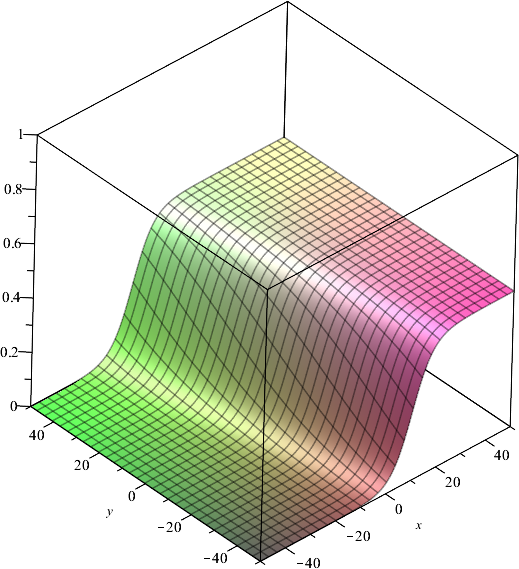
\includegraphics[width=.3\textwidth]{fig/(2+1)BKP-T-1-soliton.png}
}
\subfigure[1-soliton of BKP \label{bkp:1-soliton}]{
    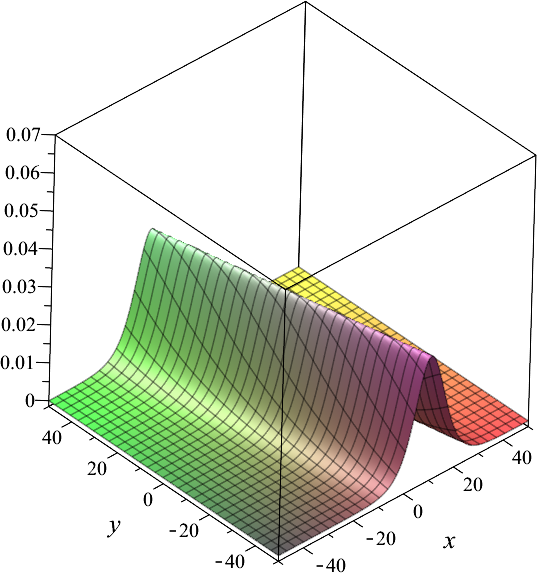
\includegraphics[width=.3\textwidth]{fig/(2+1)BKP-1-soliton.png}
}
\subfigure[2-soliton of BKP \label{bkp:2-soliton}]{
    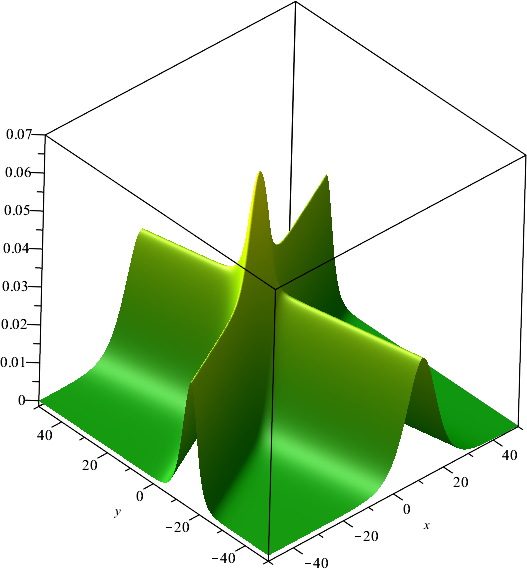
\includegraphics[width=.3\textwidth]{fig/(2+1)BKP-2-soliton.png}
}
\caption{Solitons of (2+1)BKP/BKP-T equation}\label{bkp}
\end{figure}

\section{Experiments and examples}\label{Examples-01}
Since $\PS$ is a critical object in our algorithm, several typical NLEEs are considered and solved with different $\PS$ to show the relation between $\PS$ and equation to be solved. The experiment results are shown in \reftab{verify}.

\begin{table}[htbp]
\centering 
\caption{Solution verification results} \label{verify}
\small
\begin{tabular}{lrcccc}
\hline
\multicolumn{1}{c}{Equation Name}&\multicolumn{1}{c}{$\PS$} &3-soliton &2-breather &2-lump &Error\\
\hline
(1+1)KdV &1 &\VTRUE &\VTRUE &- &err-2\\
(2+1)BKP-T &1 &\VTRUE &\VTRUE &- &err-2\\
(2+1)BKP-T &12 &\VTRUE &\VTRUE &\VTRUE &\\
(2+1)CBS &1 &\VTRUE &\VTRUE &- &err-2\\
(2+1)CBS &12 &\VTRUE &\VTRUE &- &err-3\\
(2+1)CBS-G &1 &\VTRUE &\VTRUE &- &err-2\\
(2+1)CBS-G &12 &\VFALSE &\VFALSE &\VFALSE &\\
(2+1)KP &1 &\VTRUE &\VTRUE &- &err-2\\
(2+1)KP &12 &\VTRUE &\VTRUE &\VTRUE &\\
(2+1)SK &1 &\VTRUE &\VTRUE &- &err-2\\
(2+1)SK &12 &\VTRUE &\VTRUE &\VTRUE &\\
(3+1)BKP &1 &\VTRUE &\VTRUE &- &err-2\\
(3+1)BKP &12 &\VTRUE &\VTRUE &\VTRUE &\\
(3+1)BKP &13 &\VTRUE &\VTRUE &\VTRUE &\\
(3+1)BKP &123 &\VFALSE &\VFALSE &\VFALSE &\\
(3+1)CBS &1 &\VTRUE &\VTRUE &- &err-2\\
(3+1)CBS &12 &\VTRUE &\VTRUE &- &err-3\\
(3+1)CBS &13 &\VTRUE &\VTRUE &- &err-3\\
(3+1)CBS &123 &\VTRUE &\VTRUE &- &err-3\\
(3+1)JM &1 &\VTRUE &\VTRUE &- &err-2\\
(3+1)JM &12 &\VTRUE &\VTRUE &\VTRUE &\\
(3+1)JM &13 &\VTRUE &\VTRUE &- &err-3\\
(3+1)JM &123 &\VFALSE &\VFALSE &\VFALSE &\\
(3+1)KP &1 &\VTRUE &\VTRUE &- &err-2\\
(3+1)KP &12 &\VTRUE &\VTRUE &\VTRUE &\\
(3+1)KP &13 &\VTRUE &\VTRUE &\VTRUE &\\
(3+1)KP &123 &\VFALSE &\VFALSE &\VFALSE &\\
(3+1)NEE-T &1 &\VTRUE &\VTRUE &- &err-2\\
(3+1)NEE-T &12 &\VTRUE &\VTRUE &\VTRUE &\\
(3+1)NEE-T &13 &\VTRUE &\VTRUE &- &err-3\\
(3+1)NEE-T &123 &\VFALSE &\VFALSE &\VFALSE &\\
(3+1)YTSF &1 &\VTRUE &\VTRUE &- &err-2\\
(3+1)YTSF &12 &\VTRUE &\VTRUE &\VTRUE &\\
(3+1)YTSF &13 &\VTRUE &\VTRUE &- &err-3\\
(3+1)YTSF &123 &- &- &- &err-1\\
(4+1)Fokas-T &1 &\VTRUE &\VTRUE &- &err-2\\
(4+1)Fokas-T &12 &\VTRUE &\VTRUE &- &err-3\\
(4+1)Fokas-T &13 &\VTRUE &\VTRUE &- &err-3\\
(4+1)Fokas-T &123 &\VFALSE &\VFALSE &\VFALSE &\\
(4+1)Fokas-T-2 &1 &\VTRUE &\VTRUE &- &err-2\\
(4+1)Fokas-T-2 &12 &\VTRUE &\VTRUE &\VTRUE &\\
\hline
\multicolumn{6}{l}{\pbox{0.8\textwidth}{
{\tiny ~}\\
Note:\\
err-1: $h_{i,j}$ has no solution.\\
err-2: lump solution requires that $\{1\}\subsetneq \PS$.\\
err-3: numeric exception: divided by zero.\\
其它公式见 \reftab{eqs}.
}}
\end{tabular}
\end{table}

\begin{table}[htbp]
\centering
\caption{List of equation expressions}\label{eqs}
\renewcommand{\arraystretch}{1.2}
\begin{tabular}{lp{0.7\textwidth}}
\hline
\multicolumn{1}{c}{Equation Name} & \multicolumn{1}{c}{Expression} \\
\hline
(2+1) SK\CITEbaSK & $5\,{u_{{x}}}^{2}u_{{{\it xx}}}+5\,u_{{x}}u_{{{\it xxxx}}}+5\,u_{{x}}u_{{{\it xy}}}+5\,u_{{{\it xx}}}u_{{{\it xxx}}}+5\,u_{{{\it xx}}}u_{{y}}-u_{{{\it tx}}}+u_{{{\it xxxxxx}}}+5\,u_{{{\it xxxy}}}-5\,u_{{{\it yy}}}=0$.\\
(2+1) KP\CITEbaKP & $\alpha\,u_{{{\it yy}}}+6\,uu_{{{\it xx}}}+6\,{u_{{x}}}^{2}+u_{{{\it tx}}}+u_{{{\it xxxx}}}=0$.\\
(2+1) CBS\CITEbaCBS & $4\,u_{{x}}u_{{{\it xy}}}+2\,u_{{{\it xx}}}u_{{y}}+u_{{{\it tx}}}+u_{{{\it xxxy}}}=0$.\\
(2+1) CBS-G\CITEbaCBSG & $\alpha\,u_{{{\it xy}}}+\beta\,u_{{{\it yy}}}+3\,u_{{x}}u_{{{\it xy}}}+3\,u_{{{\it xx}}}u_{{y}}+u_{{{\it tx}}}+u_{{{\it xxxy}}}=0$.\\
(3+1) CBS\CITEcaCBS & $4\,u_{{x}}u_{{{\it xy}}}+4\,u_{{x}}u_{{{\it xz}}}+2\,u_{{{\it xx}}}u_{{y}}+2\,u_{{{\it xx}}}u_{{z}}+u_{{{\it tx}}}+u_{{{\it xxxy}}}+u_{{{\it xxxz}}}=0$.\\
(3+1) BKP\CITEcaBKP & $-3\,u_{{x}}u_{{{\it xy}}}-3\,u_{{{\it xx}}}u_{{y}}+u_{{{\it ty}}}+3\,u_{{{\it xx}}}-u_{{{\it xxxy}}}+3\,u_{{{\it zz}}}=0$.\\
(3+1) KP\CITEcaKP & $-6\,uu_{{{\it xx}}}-6\,{u_{{x}}}^{2}+u_{{{\it tx}}}+u_{{{\it xxxx}}}+3\,u_{{{\it yy}}}+3\,u_{{{\it zz}}}=0$.\\
(3+1) NEE\CITEcaNEE & $3\,u_{{{\it xz}}}-2\,u_{{{\it ty}}}-u_{{{\it xxxy}}}+4\,u_{{x}}u_{{y}}+2\,uu_{{{\it xy}}}+2\,u_{{{\it xx}}}\int \!u_{{y}}\,{\rm d}x=0$.\\
(3+1) NEE-T\CITEcaNEET & $2\,v_{{x}}v_{{{\it xxy}}}+4\,v_{{{\it xx}}}v_{{{\it xy}}}+2\,v_{{{\it xxx}}}v_{{y}}-2\,v_{{{\it txy}}}-v_{{{\it xxxxy}}}+3\,v_{{{\it xxz}}}=0$.\\
(3+1) YTSF\CITEcaYTSF & $3\,\alpha\,u_{{{\it yy}}}+4\,u_{{x}}u_{{{\it xz}}}+2\,u_{{{\it xx}}}u_{{z}}-4\,u_{{{\it tx}}}+u_{{{\it xxxz}}}=0$.\\

\hline
\end{tabular}
\end{table}

In \reftab{verify}, the first column is the name of the considered equation. The postfix `-T' means transformed,  and the postfix `-G' means generalized. The second column is the abbreviation of $\PS$. For example `12' means $\PS=\{1,2\}$. Our tests omit the constant term in the travelling wave variable, because it doesn't affect the verification result.

Since 1-soliton and 2-soliton are solved directly by the undetermined coefficient method, they must meet the original equation. 
It is unnecessary to verify them, so do 1-breather and 1-lump solutions. We need to verify 3-soliton, 2-breather and 2-lump solutions. Here `\VTRUE' means that the solution meets the input equation and `\VFALSE' means that the solution fails. In addition, `-' means that the solution cannot be obtained by our method, and the reason is given in the last column. 

As we can see from \reftab{verify}, for all equations in our test, $\PS=\{1\}$ can generate genuine soliton and breather solutions. 

For most (2+1)-dimensional equations, $\PS= \ALLP$ can generate genuine solutions if it exists except for (2+1)GBS-G equation. (2+1)CBS and (2+1)GBS-G have no lump solution. 

For most (3+1)-dimensional equations in our test, $\PS= \ALLP$ cannot generate genuine soliton solutions, except for the (3+1)CBS equation. For these equations which don't have genuine solutions when $\PS= \ALLP$, have genuine solutions when $\PS=\{1,2\}$ or $\PS=\{1,3\}$. In fact, they have genuine solutions when $(p_i,q_i)~(i=1,2,\cdots)$ are linear dependent.

The (2+1)BKP-T equation and (2+1)NEE-T equation are transformed from the original equation by eliminating integral.  

In addition, dimensionality reduction is also an important technique to extend our method to higher dimensions. The (4+1)Fokas equation \CITEdaFokas{} is a typical example. The expression of this equation is 
\begin{equation}
    u_{tx}-\frac{1}{4}u_{xxxy}+\frac{1}{4}u_{xyyy}+3u_xu_y+3uu_{xy}-\frac{3}{2}u_{wz}=0. \label{Fokas}
\end{equation}
It can be solved directly by our method when $\PS=\{1,3,4\}$. The corresponding TPE is
\begin{equation}
u={\frac {{f_{{x}}}^{2}-{f_{{y}}}^{2}}{{f}^{2}}}+{\frac { \left( -5\,f_{
{{ xx}}}+f_{{{ yy}}} \right) {f_{{x}}}^{2}+8\,f_{{x}}f_{{y}}f_{{
{ xy}}}+{f_{{y}}}^{2} \left( f_{{{ xx}}}-5\,f_{{{ yy}}}
\right) }{5f(f_x^2-f_y^2)}}.
\end{equation}
But calculate the corresponding $\omega$ and $h_{i,j}$ is quite slow. It takes about 90 seconds in our experiment. The time spending on solution verification is unacceptable.

The TPE of this equation is the function w.r.t. $f,f_x$ and $f_y$, we apply the travelling wave transformation $\xi=ax+by$, and get
\begin{equation}
    au_{t\xi}-\frac{a^3b}{4}u_{\xi\xi\xi\xi}+\frac{ab^3}{4}u_{\xi\xi\xi\xi}+3abu_{\xi}^2+3abuu_{\xi\xi}-\frac{3}{2}u_{wz}=0.  \label{Fork-T}
\end{equation}
This equation is denoted as Fokas-T in \reftab{verify}. By reducing to (3+1)-dimension, the  corresponding TPE becomes
\begin{equation}
    u=(a^2-b^2)\sbrace{\frac{f_{\xi}^2}{f^2}-\frac{f_{\xi\xi}}{f}}.
\end{equation}
Assume $\PS=\{1,2,3\}$, we get
\begin{equation}
\begin{split}
    \omega&={\frac {{a}^{3}b{k}^{2}-a{b}^{3}{k}^{2}+6\,pq}{4a}}, \\
    h_{{i,j}}&={\frac {b \left( k_{{i}}-k_{{j}} \right) ^{2}{a}^{3}-{b}^{3}
    \left( k_{{i}}-k_{{j}} \right) ^{2}a-2\, \left( q_{{i}}-q_{{j}}
    \right)  \left( p_{{i}}-p_{{j}} \right) }{b \left( k_{{i}}+k_{{j}}
    \right) ^{2}{a}^{3}-{b}^{3} \left( k_{{i}}+k_{{j}} \right) ^{2}a-2\,
    \left( q_{{i}}-q_{{j}} \right)  \left( p_{{i}}-p_{{j}} \right) }}.
\end{split}
\end{equation}
As we can see from \reftab{verify}, in this case no solution meets the input equation when $\PS=\{1,2,3\}$. But they become genuine solutions when $(p_i,q_i)~(i=1,2,\cdots)$ are linear dependent.

Based on this observation, we apply the transformation $\eta=cw+dz$ to \refeqn{Fork-T}, and get
\begin{equation}
    au_{t\xi}-\frac{a^3b}{4}u_{\xi\xi\xi\xi}+\frac{ab^3}{4}u_{\xi\xi\xi\xi}+3abu_{\xi}^2+3abuu_{\xi\xi}-\frac{3cd}{2}u_{\eta\eta}=0.  \label{Fokas-T-2}
\end{equation}
This equation is denoted as Fokas-T-2 in \reftab{verify}. The key parameters of this equation are
\begin{equation}
\begin{split}
    \omega&={\frac {{a}^{3}b{k}^{2}-a{b}^{3}{k}^{2}+6\,cd{p}^{2}}{4a}}, \\ 
    h_{{i,j}}&={\frac {b \left( k_{{i}}-k_{{j}} \right) ^{2}{a}^{3}-{b}^{3}
    \left( k_{{i}}-k_{{j}} \right) ^{2}a-2\,cd \left( p_{{i}}-p_{{j}}
    \right) ^{2}}{b \left( k_{{i}}+k_{{j}} \right) ^{2}{a}^{3}-{b}^{3}
    \left( k_{{i}}+k_{{j}} \right) ^{2}a-2\,cd \left( p_{{i}}-p_{{j}}
    \right) ^{2}}}.
\end{split}
\end{equation}
As we can see from \reftab{verify}, in this case all obtained solutions meet the input equation.

The runtime of verifying all solutions is summarized in \reftab{runtime}. It can be seen that method-1 is the most efficient in general. The verification of 2-breather solutions takes the most time. So method-1 is the best choice of solution verification. Thus, \texttt{method=1} is the default value in our package. 

\begin{table}[htbp]
\centering 
\caption{Summary of runtime} \label{runtime}
\begin{tabular}{c|ccc|c}
\hline
time(h) &method-1 &method-2 &method-3 &sum\\
\hline
solve &0.002 &0.002 &0.002 &0.005\\
3-soliton &0.002 &0.002 &0.016 &0.020\\
2-breather &0.212 &0.949 &1.551 &2.713\\
2-lump &0.022 &0.022 &0.033 &0.077\\
\hline
sum &0.238 &0.975 &1.602 &2.815\\

\hline
\end{tabular}
\end{table}

\section{Conclusions}\label{Conclusions-01}
Based on the simplified Hirota method, conjugate parameter assignment and long wave limit method, we propose a novel algorithm that can derive possible soliton, breather and lump solutions to NLEEs automatically. For convenience to program and further generalization, we made the following improvements:
\begin{compactitem}[\textbullet]
\item Introduce $\PS$ for getting genuine solutions of non-integrable equations.
\item Infer the computation formula of key parameters for lump solutions in general cases.
\item Rewrite the generate formula of soliton and lump solutions for the convenience to program. 
\end{compactitem}

As the dimension increases, equations usually are non-integrable. In order to get genuine solution by our method, here are some useful techniques:
\begin{compactitem}[\textbullet]
\item Adopt proper subset $\PS\subsetneq  \ALLP$. 
\item Consider linear correlation between parameters.
\item Dimensionality reduction.
\end{compactitem}

Finally, the implemented Maple package \texttt{TwSolver} provides convenient interfaces for solving, verifying and plotting.
